\documentclass[a4paper,12pt]{article}

% ── Fonts ─────────────────────────────────────────────────────────────────────
\usepackage[T1]{fontenc}
\usepackage[scaled=1.0]{helvet}      % Arial-equivalent (Helvetica)
\renewcommand{\familydefault}{\sfdefault}
\usepackage{microtype}               % Better typography

% ── Page geometry ─────────────────────────────────────────────────────────────
\usepackage[
  a4paper,
  top=25mm, bottom=25mm,
  left=25mm, right=25mm,
  headheight=14pt
]{geometry}

% ── Essential packages ─────────────────────────────────────────────────────────
\usepackage{ragged2e}                % \justifying
\usepackage{setspace}
\usepackage{parskip}
\usepackage{graphicx}
\usepackage{xcolor}
\usepackage{enumitem}
\usepackage{booktabs}
\usepackage{tabularx}
\usepackage{array}
\usepackage{fancyhdr}
\usepackage{titlesec}
\usepackage{hyperref}
\usepackage{mdframed}
\usepackage{tikz}
\usetikzlibrary{shapes.geometric, arrows.meta, positioning, fit, backgrounds}

% ── Colors ────────────────────────────────────────────────────────────────────
\definecolor{sapblue}{RGB}{10, 110, 209}
\definecolor{darkgray}{RGB}{50, 54, 58}
\definecolor{lightgray}{RGB}{242, 242, 242}
\definecolor{accentgreen}{RGB}{16, 126, 62}
\definecolor{accentorange}{RGB}{233, 115, 12}
\definecolor{boxbg}{RGB}{235, 244, 255}

% ── Section formatting  (15pt heading / 14pt subheading) ──────────────────────
\titleformat{\section}
  {\fontsize{15}{18}\bfseries\color{sapblue}}
  {\thesection.}{0.5em}{}
\titleformat{\subsection}
  {\fontsize{14}{17}\bfseries\color{darkgray}}
  {\thesubsection}{0.5em}{}
\titleformat{\subsubsection}
  {\fontsize{12}{15}\bfseries\color{darkgray}}
  {}{0em}{}

% ── Page style ─────────────────────────────────────────────────────────────────
\pagestyle{fancy}
\fancyhf{}
\renewcommand{\headrulewidth}{0.4pt}
\fancyhead[L]{\small\color{darkgray}Order-to-Cash (O2C) — SAP BTP Capstone Project}
\fancyhead[R]{\small\color{darkgray}KIIT}
\fancyfoot[R]{\small\thepage}          % page number bottom-right

% ── Hyperlinks ─────────────────────────────────────────────────────────────────
\hypersetup{
  colorlinks=true,
  linkcolor=sapblue,
  urlcolor=sapblue,
  pdfauthor={KIIT Student},
  pdftitle={O2C SAP BTP Capstone Project Report}
}

% ── Justified text ──────────────────────────────────────────────────────────────
\setlength{\parindent}{0pt}
\setlength{\parskip}{6pt}

\begin{document}
\justifying
\setstretch{1.15}

% ══════════════════════════════════════════════════════════════════════════════
%  TITLE PAGE
% ══════════════════════════════════════════════════════════════════════════════
\thispagestyle{empty}

\begin{center}
  \vspace*{10mm}

  {\color{sapblue}\rule{\linewidth}{2pt}}
  \vspace{6mm}

  {\fontsize{22}{28}\bfseries\color{sapblue}
    Order-to-Cash (O2C)\\[4pt]
    SAP Cloud Application Programming Model}
  \vspace{4mm}

  {\fontsize{15}{20}\bfseries\color{darkgray} Capstone Project Report}
  \vspace{2mm}

  {\color{sapblue}\rule{\linewidth}{2pt}}
  \vspace{12mm}

  \begin{tabular}{rl}
    \textbf{Program}     & SAP Business Technology Platform (BTP) \\[4pt]
    \textbf{Institute}   & KIIT \\[4pt]
    \textbf{Submitted On} & \today \\
  \end{tabular}

  \vspace{16mm}

  % Process flow visual on title page
  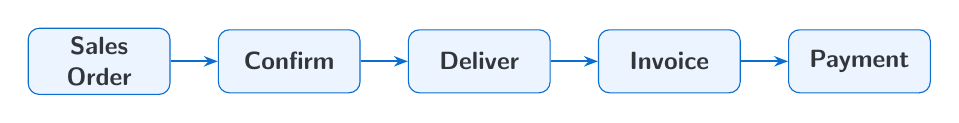
\begin{tikzpicture}[
      box/.style={
        rectangle, rounded corners=4pt,
        minimum width=1.8cm, minimum height=0.8cm,
        draw=sapblue, fill=boxbg, font=\small\bfseries, text=darkgray,
        align=center
      },
      arr/.style={-{Stealth[length=5pt]}, thick, color=sapblue}
  ]
    \node[box] (so)  {Sales\\Order};
    \node[box] (cf)  [right=0.6cm of so] {Confirm};
    \node[box] (del) [right=0.6cm of cf] {Deliver};
    \node[box] (inv) [right=0.6cm of del] {Invoice};
    \node[box] (pay) [right=0.6cm of inv] {Payment};

    \draw[arr] (so)  -- (cf);
    \draw[arr] (cf)  -- (del);
    \draw[arr] (del) -- (inv);
    \draw[arr] (inv) -- (pay);
  \end{tikzpicture}

  \vspace{6mm}
  {\small\color{darkgray}\itshape
    ``Automating the complete sales lifecycle — from customer order to cash receipt''}
\end{center}

\newpage
\setcounter{page}{1}

% ══════════════════════════════════════════════════════════════════════════════
%  1. PROBLEM STATEMENT
% ══════════════════════════════════════════════════════════════════════════════
\section{Problem Statement}

In modern enterprises, the \textbf{Order-to-Cash (O2C)} process spans multiple departments — sales, warehouse, logistics, and finance — often resulting in disconnected workflows, manual handoffs, and delayed revenue recognition. Without a unified digital system, organizations face challenges such as:

\begin{itemize}[leftmargin=1.5em, itemsep=3pt]
  \item Inability to track an order's real-time status across departments.
  \item Manual, error-prone invoice generation leading to billing disputes.
  \item No automated credit-limit checks before order confirmation, increasing financial risk.
  \item Stock inconsistencies caused by uncoordinated order confirmation and warehouse operations.
  \item Fragmented payment records making cash flow visibility difficult for finance teams.
\end{itemize}

The goal of this project is to design and develop a \textbf{cloud-native O2C application on SAP BTP} using the SAP Cloud Application Programming (CAP) model. The system must enforce the complete business process from sales order creation through to payment collection, applying business rules at every stage — all exposed via a standards-compliant OData v4 API and a browser-based dashboard.

% ══════════════════════════════════════════════════════════════════════════════
%  2. SOLUTION AND FEATURES
% ══════════════════════════════════════════════════════════════════════════════
\section{Solution and Features}

\subsection{Solution Overview}

The application implements the O2C cycle as a five-stage stateful workflow. Each stage is guarded by business rule validations and exposed as an OData action. The backend is built using \textbf{SAP CAP (Node.js)} with SQLite for local development and is designed for deployment to \textbf{SAP HANA Cloud} on BTP. The frontend is a single-page Fiori-styled dashboard that provides a complete operational view.

\subsection{Key Features}

\begin{itemize}[leftmargin=1.5em, itemsep=4pt]
  \item \textbf{Sales Order Management} — Create, view, and manage sales orders with automatic order-number generation, multi-line item support, and real-time total calculation.

  \item \textbf{Line Item Pricing Engine} — Unit prices and GST rates are auto-populated from the product master at the time of order creation. Per-line discount support with automatic net, tax, and total computations.

  \item \textbf{Order Confirmation with Business Rules} — Confirmation validates that the order has at least one line item, and performs a \textit{credit limit check} against the customer master before allowing the transition from \texttt{Draft} to \texttt{Confirmed}. Stock is atomically deducted on confirmation.

  \item \textbf{Delivery Lifecycle} — A delivery document is created for Confirmed orders and progresses through \texttt{Pending} → \texttt{Shipped} (with tracking number) → \texttt{Delivered} stages.

  \item \textbf{Automated Invoice Generation} — Invoices are generated for Delivered orders. Invoice amounts are derived directly from the sales order; due date is set to 30 days from the invoice date. Duplicate invoice prevention is enforced.

  \item \textbf{Payment Recording} — Finance teams record payment references against open invoices. On payment, the parent sales order is automatically moved to \texttt{Paid} status.

  \item \textbf{Order Cancellation with Stock Reversal} — Draft and Confirmed orders can be cancelled. Stock that was deducted on confirmation is automatically returned to inventory.

  \item \textbf{Dashboard KPIs} — A real-time summary groups orders by status with count and revenue aggregation, giving management instant visibility into pipeline health.
\end{itemize}

% ══════════════════════════════════════════════════════════════════════════════
%  3. SYSTEM ARCHITECTURE
% ══════════════════════════════════════════════════════════════════════════════
\section{System Architecture}

\subsection{High-Level Architecture}

\begin{center}
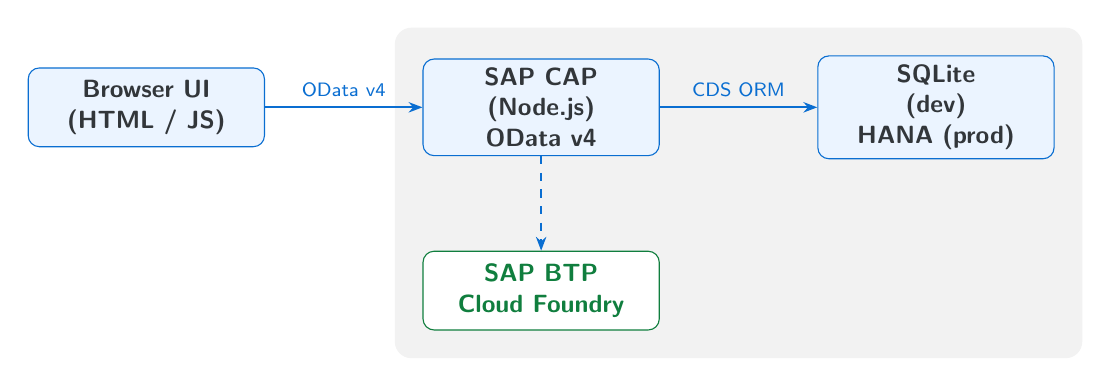
\begin{tikzpicture}[
    box/.style={
      rectangle, rounded corners=4pt, draw=sapblue,
      minimum width=3cm, minimum height=1cm,
      align=center, font=\small\bfseries, fill=boxbg, text=darkgray
    },
    cloud/.style={
      box, fill=white, draw=accentgreen, text=accentgreen
    },
    arr/.style={-{Stealth[length=5pt]}, thick, color=sapblue}
]
  \node[box]   (ui)    {Browser UI\\(HTML / JS)};
  \node[box]   (cap)   [right=2cm of ui] {SAP CAP\\(Node.js)\\OData v4};
  \node[box]   (db)    [right=2cm of cap] {SQLite\\(dev)\\HANA (prod)};
  \node[cloud] (btp)   [below=1.2cm of cap] {SAP BTP\\Cloud Foundry};

  \draw[arr] (ui)  -- node[above,font=\scriptsize]{OData v4} (cap);
  \draw[arr] (cap) -- node[above,font=\scriptsize]{CDS ORM} (db);
  \draw[arr,dashed] (cap) -- (btp);

  \begin{pgfonlayer}{background}
    \node[fill=lightgray, rounded corners=6pt, inner sep=10pt,
          fit=(cap)(db)(btp)] {};
  \end{pgfonlayer}
\end{tikzpicture}
\end{center}

\subsection{Backend Layer Design (CAP Layered Architecture)}

The backend follows the standard CAP layered approach:

\begin{center}
\begin{tabular}{>{\bfseries\color{sapblue}}p{3.5cm} p{9cm}}
\toprule
Layer & Responsibility \\
\midrule
\texttt{db/schema.cds}     & Entity definitions, relationships, type enums \\
\texttt{srv/*.cds}         & OData service exposure, action/function signatures \\
\texttt{srv/*.js}          & Custom event handlers — business logic, validation \\
\texttt{db/data/*.csv}     & Seed data for SQLite (Customers, Products) \\
\texttt{app/webapp/}       & Fiori-styled HTML dashboard \\
\texttt{test/}             & Jest end-to-end test suite \\
\bottomrule
\end{tabular}
\end{center}

\subsection{Data Model (Entity Relationship)}

Six core entities model the O2C process:

\begin{itemize}[leftmargin=1.5em, itemsep=2pt]
  \item \texttt{Customers} — master record with credit limit
  \item \texttt{Products} — material master with pricing and GST rate
  \item \texttt{SalesOrders} — central document linking all stages; carries lifecycle status
  \item \texttt{SalesOrderItems} — line items with auto-calculated pricing
  \item \texttt{Deliveries} — one-to-one with a Sales Order; tracks shipment
  \item \texttt{Invoices} — one-to-one with a Sales Order; tracks payment
\end{itemize}

\newpage

% ══════════════════════════════════════════════════════════════════════════════
%  4. TECH STACK
% ══════════════════════════════════════════════════════════════════════════════
\section{Technology Stack}

\begin{center}
\begin{tabularx}{\linewidth}{>{\bfseries}l >{\raggedright\arraybackslash}X l}
\toprule
Component & Technology & Version \\
\midrule
CAP Framework & SAP Cloud Application Programming Model & 7.x \\
Runtime & Node.js & 18 LTS+ \\
Data Modelling & CDS (Core Data Services) & — \\
OData & Auto-generated OData v4 service & v4 \\
Database (Dev) & SQLite (in-memory) & — \\
Database (Prod) & SAP HANA Cloud & — \\
Frontend & HTML5, Vanilla JS, Fiori Design System CSS & — \\
Testing & Jest + \texttt{cds.test} + Supertest & 29.x \\
Version Control & Git / GitHub & — \\
Deployment & SAP BTP Cloud Foundry & — \\
\bottomrule
\end{tabularx}
\end{center}

% ══════════════════════════════════════════════════════════════════════════════
%  5. O2C PROCESS FLOW (Screenshots / Functional Walkthrough)
% ══════════════════════════════════════════════════════════════════════════════
\section{Process Flow Walkthrough}

The following diagram illustrates the complete O2C lifecycle with enforced state transitions and the business rules applied at each step:

\begin{center}
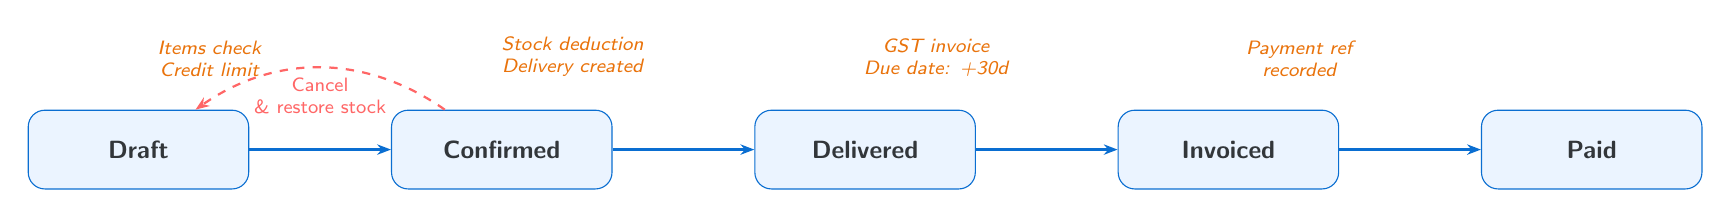
\begin{tikzpicture}[
    state/.style={
      rectangle, rounded corners=6pt, draw=sapblue, fill=boxbg,
      minimum width=2.8cm, minimum height=1cm, align=center,
      font=\small\bfseries, text=darkgray
    },
    rule/.style={font=\scriptsize\itshape, color=accentorange, align=center, text width=2.5cm},
    arr/.style={-{Stealth[length=5pt]}, thick, color=sapblue}
]
  \node[state]              (draft)     {Draft};
  \node[state, right=1.8cm of draft]   (confirmed) {Confirmed};
  \node[state, right=1.8cm of confirmed] (delivered) {Delivered};
  \node[state, right=1.8cm of delivered] (invoiced)  {Invoiced};
  \node[state, right=1.8cm of invoiced]  (paid)      {Paid};

  % Arrows
  \draw[arr] (draft) -- (confirmed);
  \draw[arr] (confirmed) -- (delivered);
  \draw[arr] (delivered) -- (invoiced);
  \draw[arr] (invoiced) -- (paid);

  % Rule labels above arrows
  \node[rule, above=0.3cm of draft, xshift=0.9cm]
    {Items check\\Credit limit};
  \node[rule, above=0.3cm of confirmed, xshift=0.9cm]
    {Stock deduction\\Delivery created};
  \node[rule, above=0.3cm of delivered, xshift=0.9cm]
    {GST invoice\\Due date: +30d};
  \node[rule, above=0.3cm of invoiced, xshift=0.9cm]
    {Payment ref\\recorded};

  % Cancel path
  \draw[arr, dashed, color=red!60]
    (confirmed) to[bend right=35]
    node[below, font=\scriptsize\color{red!70}, align=center]{Cancel\\\&\ restore stock}
    (draft);
\end{tikzpicture}
\end{center}

\textbf{Step-by-step flow:}

\begin{enumerate}[leftmargin=1.8em, itemsep=4pt]
  \item \textbf{Sales Order (Draft)} — A sales representative creates the order, selects the customer, and adds line items. Prices and GST auto-fill from the product master.
  \item \textbf{Confirm Order} — The system checks credit limit and item presence, then deducts stock. Status moves to \texttt{Confirmed}.
  \item \textbf{Create Delivery} — Warehouse creates a delivery document with planned date and carrier. Status moves to \texttt{Delivered} on the sales order.
  \item \textbf{Generate Invoice} — Finance generates the invoice; amounts are copied from the order. Due date is set to 30 days ahead.
  \item \textbf{Record Payment} — Finance records the payment reference (bank transfer / cheque). Invoice is marked paid; order status becomes \texttt{Paid}.
\end{enumerate}

% ══════════════════════════════════════════════════════════════════════════════
%  6. UNIQUE POINTS
% ══════════════════════════════════════════════════════════════════════════════
\section{Unique Points}

\begin{enumerate}[leftmargin=1.8em, itemsep=5pt]
  \item \textbf{OData v4 Native API} — The entire application is exposed as a fully standards-compliant OData v4 service. This means it can be consumed directly by SAP Fiori Elements, Power BI, or any OData-capable client without any additional API layer.

  \item \textbf{Strict State Machine Enforcement} — Every stage transition is validated server-side. There is no way to, for instance, invoice an order that has not been delivered — the business process integrity is guaranteed by the service layer, not just the UI.

  \item \textbf{Atomic Stock Management} — Stock deduction (on confirmation) and restoration (on cancellation) happen within the same database transaction, eliminating the possibility of stock inconsistencies under concurrent access.

  \item \textbf{GST-Aware Pricing Engine} — Each line item carries its own tax rate (sourced from the product master), and tax amounts are computed and stored separately from net amounts — making the invoices audit-ready and GST-compliant.

  \item \textbf{CAP Portability} — By switching one configuration entry in \texttt{package.json} from \texttt{sqlite} to \texttt{hana}, the entire application is ready to deploy against SAP HANA Cloud on BTP without changing a single line of business logic.

  \item \textbf{Comprehensive Test Coverage} — The project includes 15 automated tests covering all happy paths, error paths, and duplicate-prevention checks, using the official \texttt{cds.test} harness.
\end{enumerate}

% ══════════════════════════════════════════════════════════════════════════════
%  7. FUTURE IMPROVEMENTS
% ══════════════════════════════════════════════════════════════════════════════
\section{Future Improvements}

\begin{itemize}[leftmargin=1.5em, itemsep=4pt]
  \item \textbf{SAP Fiori Elements UI} — Replace the hand-coded HTML dashboard with a metadata-driven Fiori Elements application (List Report + Object Page floor plan) for a native SAP UX experience.

  \item \textbf{SAP Event Mesh Integration} — Publish O2C lifecycle events (order confirmed, invoice generated) to SAP Event Mesh, enabling other BTP services (e.g., an analytics microservice) to react asynchronously.

  \item \textbf{Role-Based Access Control} — Implement SAP BTP XSUAA authentication and define roles such as \textit{SalesRep}, \textit{Warehouse}, and \textit{Finance} so that each persona only sees and performs actions relevant to their stage.

  \item \textbf{PDF Invoice Generation} — Integrate a PDF generation service to produce formatted, downloadable invoice PDFs directly from the application.

  \item \textbf{Multi-Currency Support} — Extend the pricing model to support transactions in multiple currencies with exchange-rate lookups from an SAP currency conversion service.

  \item \textbf{SAP Analytics Cloud Dashboard} — Expose O2C KPI data to SAP Analytics Cloud (SAC) for executive-level revenue dashboards and trend analysis.

  \item \textbf{Email Notifications} — Trigger email alerts at key milestones (order confirmed, invoice due soon, payment overdue) via SAP BTP Alert Notification Service.
\end{itemize}

% ══════════════════════════════════════════════════════════════════════════════
%  8. CONCLUSION
% ══════════════════════════════════════════════════════════════════════════════
\section{Conclusion}

This project demonstrates a production-ready implementation of the Order-to-Cash business process using SAP's modern cloud-native tooling. By leveraging the SAP CAP framework, the application achieves a clean separation of concerns — the data model, service contract, and business logic are each maintained in dedicated, independently testable files. The result is a maintainable, portable, and extensible application that can serve as a foundation for a real enterprise O2C system on SAP BTP.

\vspace{8mm}
\begin{mdframed}[backgroundcolor=lightgray, roundcorner=4pt, linewidth=0pt, innertopmargin=8pt, innerbottommargin=8pt]
\textbf{GitHub Repository:} \texttt{https://github.com/<your-username>/o2c-cap-project}\\
\textbf{Submission Date:} \today \\
\textbf{Deadline:} April 21, 2026 | 11:59 PM
\end{mdframed}

\end{document}
